% -*- TeX -*- -*- UK -*- -*- Soft -*-

\chapter{Google Colaboratory}
\label{sec:Google Colaboratory}

The early content of chapter is based on material from  \cite{LiuCoLab2019,AnneBonner2019}.
\section{Background}

See the FAQ
\lstinline{https://research.google.com/colaboratory/faq.html}

It is an online  free research tool storing colab notebooks on Google Drive. Colab notebooks can import from Jupyter notebooks.

The code is executed in a virtual machine dedicated to your account. Virtual machines are recycled when idle for a while, and have a maximum lifetime enforced by the system. 

Colaboratory is intended for interactive use. Long-running background computations, particularly on GPUs, may be stopped. We encourage users who wish to run continuous or long-running computations through Colaboratory’s UI to use a local runtime, see \cite{googleLcalColabs2019}.

Colab is ideal for everything from improving your Python coding skills to working with deep learning libraries, like PyTorch, Keras, TensorFlow, and OpenCV. You can create notebooks in Colab, upload notebooks, store notebooks, share notebooks, mount your Google Drive and use whatever you’ve got stored in there, import most of your favorite directories, upload your personal Jupyter Notebooks, upload notebooks directly from GitHub, upload Kaggle files, download your notebooks, and do just about everything else that you might want to be able to do.

\section{Working with Colaboratory Notebooks}
\subsection{Getting Started}
\begin{marginfigure}
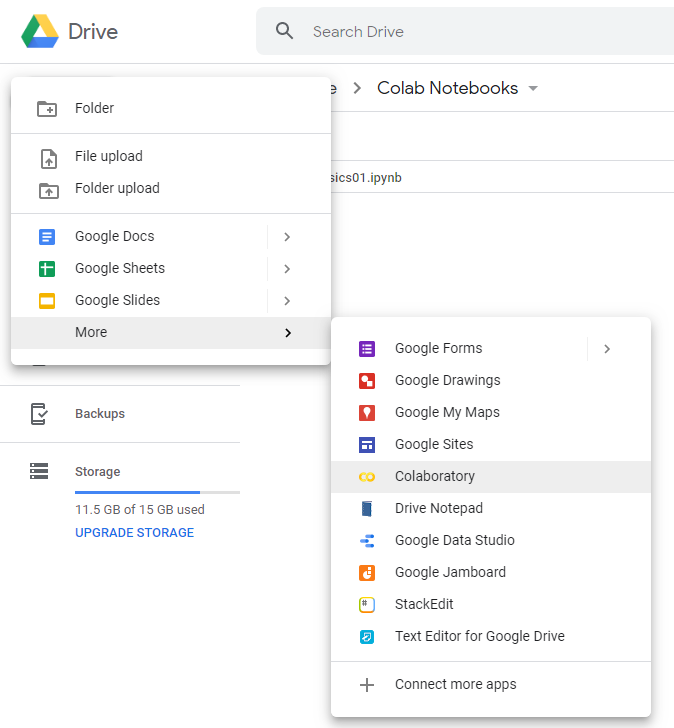
\includegraphics{drivecolab}
\end{marginfigure}
Start by making a folder in your Google Drive to store the colab notebooks and then create a new colab notebook. Note that you can also create a new notebook directly from colab itself.

Open \lstinline{https://colab.research.google.com} in a browser and click on \lstinline{NEW PYTHON 3 NOTEBOOK} in the lower right corner.  This should launch a notebook in your browser. 

Browse around and you will find lots of useful information on the welcome page.

Once you have a notebook created, it'll be saved in your Google Drive (Colab Notebooks folder). You can access it by visiting your Google Drive page, then either double-click on the file name, or right-click, and then choose ``Open with Colab''.  Alternatively you can open it from within colab from the menu by File$>$Open and then click on the Google Drive tab.

\begin{marginfigure}
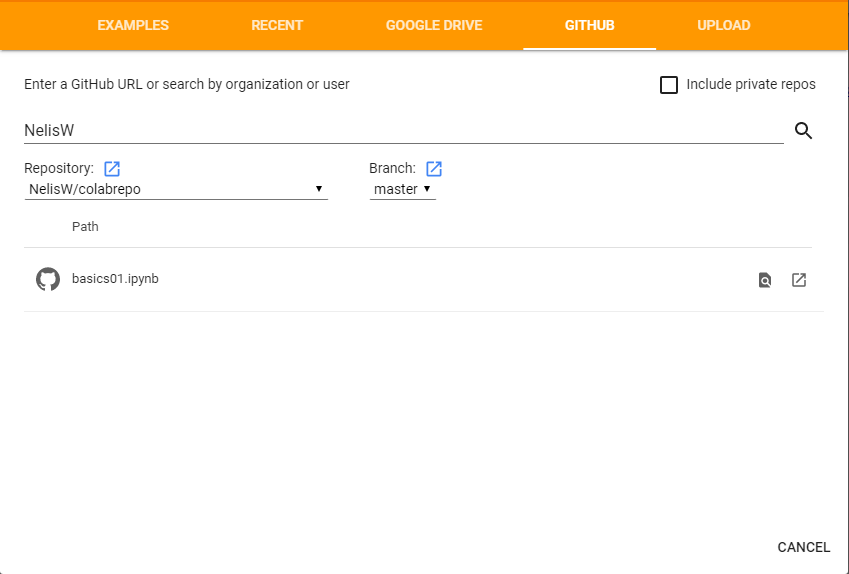
\includegraphics{drivecolab05}
\end{marginfigure}

Rename the notebook by clicking on the notebook's name or use the File$>$Rename menu.

\subsection{Connecting to a Notebook}
After some time of inactivity or after the maximum session time, Google will terminate the session.
The session can be reconnected (or changed to a local or hosted runtime) by clicking in the drop-down box in the top right of the window. Select appropriately and after some time the session will connect and a green tick mark will appear showing how much RAM and disk space are currently in use. 
\begin{marginfigure}
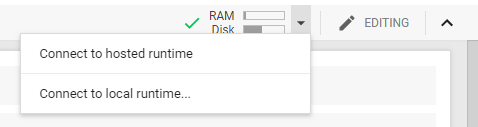
\includegraphics{drivecolab06}
\end{marginfigure}


\subsection{Saving on GitHub}

Create a new repository, and commit at least one file to the master branch, so that the github repo has a master branch (not an empy repo).
In the colab File menu select save copy to github.
You will be asked to authorise the access and henceforth it should work without further authorisation.
Select the require repository and its master branch and then click on OK.
In future, the file can be opened from within GitHub by clicking on the button.

Just be careful if saving colab notebooks, it will overwrite files by the same name in GitHub.
\begin{figure*}[h]
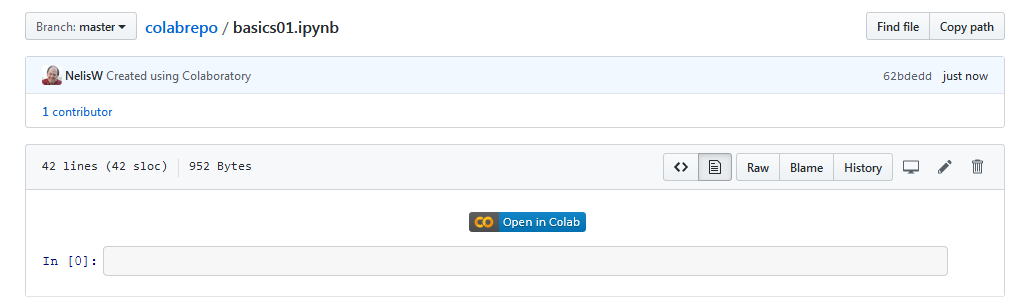
\includegraphics[width=\textwidth]{colabrepo01}
\end{figure*}


\subsection{Enabling GPU Support}

To turn on GPU for your Deep Learning projects, just go to the drop-down menu and select Runtime$>$Change runtime type$>$Hardware accelerator and choose GPU

\subsection{Working with the Notebook}

The colab notebooks are similar to Jupyter notebooks, use the same commands.
You can also save files to your colab folder (and presumably then also to github).

\subsection{Mounting Google Drive}

If you want to mount your Google Drive for file access, execute

\begin{lstlisting}
from google.colab import drive
drive.mount('/content/gdrive')
\end{lstlisting}

Google will respond by requesting you to authorise access to your user account and then its Drive services, respond by approving. You will be given an authorisation code which must be copied and pasted in the box provided. Once done, you will be informed of the mount point.
\begin{marginfigure}
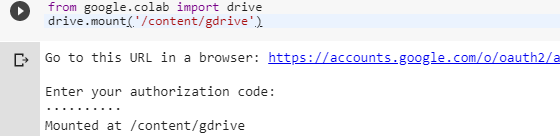
\includegraphics{drivecolab02}
\end{marginfigure}
The drive will also be visible in the Files tab on the left explorer pane.  You can list current folder's contents with the Unix 'ls' command.
\begin{marginfigure}
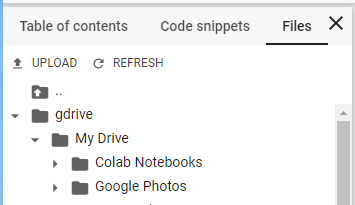
\includegraphics{drivecolab03}
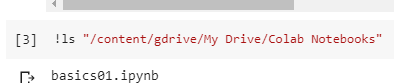
\includegraphics{drivecolab04}
\end{marginfigure}

\subsection{Uploading and Downloading Files}

Files can be uploaded by clicking on the UPLOAD button in the explorer pane.


Use wget to download and if it is a zipped file, unzip to get the contents.

\begin{lstlisting}
!wget -cq https://s3.amazonaws.com/content.udacity-data.com/courses/nd188/flower_data.zip
!unzip -qq flower_data.zip
\end{lstlisting}

\subsection{Long Running Processes}

Colaboratory is intended for interactive use. Long-running background computations, particularly on GPUs, may be stopped. ... Google encourages users who wish to run continuous or long-running computations through Colaboratory’s UI to use a local runtime or Google's paid services.




\subsection{Terminating a Session}

Virtual machines are recycled when idle for a while, and have a maximum lifetime enforced by the system.
It's 90 minutes if you close the browser. 12 hours if you keep the browser open. Additionally, if you close your browser when a code cell is running, if that same cell has not finished, when you reopen the browser it will still be running (the current executing cell keeps running even after browser is closed)
When you close the browser while a cell is still running the results will not end up saved on Google Drive.


To see a list of all the open sessions or to terminate a session on the menu click on Runtime$>$Manage sessions.  A new window will open that shows all open sessions.  The same window allows the termination of a session.
\begin{marginfigure}
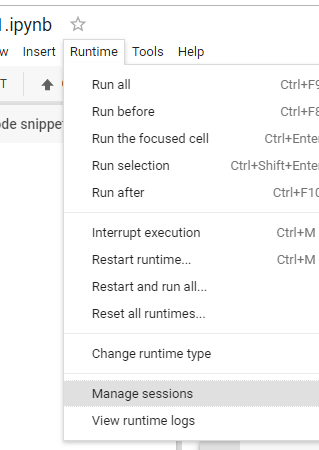
\includegraphics{drivecolab07}
\end{marginfigure}




\section{Working with Colab Notebooks}

Colab notebooks are very similar to Jupyter notebooks.
Run Python code in the same manner.

Use the ! prepend to execute system level commands such as \lstinline{!pip} or \lstinline{!apt-get install}:
\begin{lstlisting}
!pip install -q keras
import keras
\end{lstlisting}


\section{Introduction to TensorFlow}

\subsection{Tensors}

TensorFlow bases its name on the word ``tensor''. What is a tensor anyway? In short, a multi-dimensional array. Let's see what that means!

\begin{itemize}
\item We have one single number, e.g. 6, we call it a ``scalar'';
\item We have three numbers, e.g. [ 6, 8, 9], we call that a ``vector'';
\item We have a table of numbers, e.g. [[6, 8, 9], [2, 5, 7]], we call that a ``matrix'' (which has two rows and three columns);
\item We have a table of table of numbers, e.g. [[[6, 8, 9], [2, 5, 7]], [[6, 8, 9], [2, 5, 7]]], and…we are running out of words here :( My friend, that is a tensor! A tensor is just a generalized form of arrays that can have any number of dimensions.
\end{itemize}

In TensorFlow jargons, a scalar is a rank 0 tensor, a vector is rank 1 and matrix rank 2 etc. There are three frequently used types of tensors: constant, variable, and placeholder which are explained below.

\subsection{Types of Tensors}

Constants are exactly what their names refer to. They are the fixed numbers in your equation. To define a constant, we can do this:

\begin{lstlisting}[language=Python]
a = tf.constant(1, name='a_var')
b = tf.constant(2, name='b_bar')
\end{lstlisting}
Aside from the value 1, we can also provide a name such as \lstinline{a_var} for the tensor which is separate from the Python variable name \lstinline{a}. It's optional but will be helpful in later operations and troubleshooting.

After defining, if we print variable a, we'll have:

\begin{lstlisting}[language=Python]
<tf.Tensor 'a_var:0' shape=() dtype=int32>
\end{lstlisting}
Variables are the model parameters to be optimized, for example, the weights and biases in your neural networks. Similarly, we can also define a variable and show its contents like this:

\begin{lstlisting}
c = tf.Variable(a + b)
c
\end{lstlisting}
and have this output:

\begin{lstlisting}
<tf.Variable 'Variable:0' shape=() dtype=int32_ref>
\end{lstlisting}
But it's important to note that all variables need to be initialized before use like this:

\begin{lstlisting}
init = tf.global_variables_initializer()
\end{lstlisting}
You might have noticed that the values of a and b, i.e., integers 1 and 2 are not showing up anywhere, why?

That's an important characteristic of TensorFlow --- ``lazy execution'', meaning things are defined first, but not run. It's only executed when we tell it to do, which is done through the running of a session! (Note that TensorFlow also has eager execution. Check here for more info)

\subsection{Session and Computational Graph}

Now let's define a session and run it:

\begin{lstlisting}
with tf.Session() as session:                    
    session.run(init)                            
    print(session.run(c))
\end{lstlisting}
Notice that within the session we run both the initialization of variables and the calculation of c. We defined c as the sum of a and b:

\begin{lstlisting}
c = tf.Variable(a + b)
\end{lstlisting}
This, in TensorFlow and Deep Learning speak, is the ``computational graph''. Sounds pretty sophisticated, right? But it's really just an expression of the calculation we want to carry out!

\subsection{Placeholder}

Another important tensor type is the placeholder. Its use case is to hold the place for data to be supplied. For example, we defined a computational graph, and we have lots of training data, we can then use placeholders to indicate we'll feed these in later.

Let's see an example. Say we have an equation like this:

\begin{equation}
y = ax^2+bbx+c
\end{equation}

Instead of one single x input, we have a vector of x's. So we can use a placeholder to define x:

\begin{lstlisting}
x = tf.placeholder(dtype=tf.float32)
\end{lstlisting}
We also need the coefficients. Let's use constants:

\begin{lstlisting}
a = tf.constant(1, dtype=tf.float32)
b = tf.constant(-20, dtype=tf.float32)
c = tf.constant(-100, dtype=tf.float32)
\end{lstlisting}
Now let's make the computational graph and provide the input values for x:

\begin{lstlisting}
y = a * (x ** 2) + b * x + c
x_feed = np.linspace(-10, 30, num=10)
\end{lstlisting}
And finally, we can run it:

\begin{lstlisting}
with tf.Session() as sess:
  results = sess.run(y, feed_dict={x: x_feed})
print(results)
\end{lstlisting}
which gives us:

\begin{lstlisting}
[ 200.         41.975304  -76.54321  -155.55554  -195.06174  -195.06174  -155.55554   -76.54324    41.97534   200.      ]
\end{lstlisting}
\subsection{Putting it All Together}

Now that we have the basics of TensorFlow, let's do a mini project to build a linear regression model, aka, a neural network :) (The code is adapted from the example given in TensorFlow's guide here)

Let's say we have a bunch of x, y value pairs, and we need to find the best fit line. First, since both x and y have values to be fed in the model, we'll define them as placeholders:

\begin{lstlisting}
x = tf.placeholder(dtype=tf.float32, shape=(None, 1))
y_true = tf.placeholder(dtype=tf.float32, shape=(None, 1))
\end{lstlisting}
The number of rows is defined as None to have the flexibility of feeding in any number of rows we want.

Next, we need to define a model. In this case here, our model has just one layer with one weight and one bias.

\begin{marginfigure}
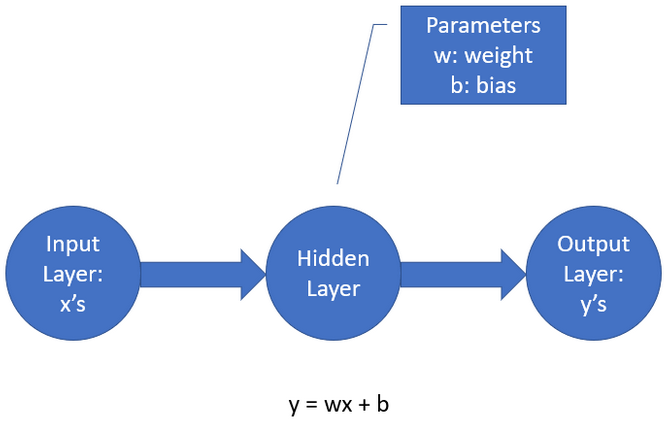
\includegraphics{colabrepo03}
\end{marginfigure}


TensorFlow allows us to define neural network layers very easily:

\begin{lstlisting}
linear_model = tf.layers.Dense(
                   units=1, 
                   bias_initializer=tf.constant_initializer(1))
y_pred = linear_model(x)
\end{lstlisting}
The number of units is set to be one since we only have one node in the hidden layer.

Furthermore, we need to have a loss function and set up the optimization method. The loss function is basically a way to measure how bad our model is when measured using the training data, so of course, we want it to be minimized. We'll use the gradient descent algorithm to optimize this loss function (I'll explain gradient descent in a future post).

\begin{lstlisting}
optimizer = tf.train.GradientDescentOptimizer(0.01)
train = optimizer.minimize(loss)
\end{lstlisting}
Then we can initialize all the variables. In this case here, all our variables including weight and bias are part of the layer we defined above.

\begin{lstlisting}
init = tf.global_variables_initializer()
\end{lstlisting}
Lastly, we can supply the training data for the placeholders and start the training:

\begin{lstlisting}
x_values = np.array([[1], [2], [3], [4]])
y_values = np.array([[0], [-1], [-2], [-3]])

with tf.Session() as sess:
  sess.run(init)
  for i in range(1000):
    _, loss_value = sess.run((train, loss),
                             feed_dict={x: x_values, y_true: y_values})
\end{lstlisting}
and we can get the weights and make the predictions like so:

\begin{lstlisting}
weights = sess.run(linear_model.weights)
bias = sess.run(linear_model.bias)
preds = sess.run(y_pred, 
                 feed_dict={x: x_values})
\end{lstlisting}
which yields these predictions:

\begin{lstlisting}
[[-0.00847495]  [-1.0041066 ]  [-1.9997383 ]  [-2.99537   ]]
\end{lstlisting}
If you are curious like me, you can verify to confirm the model did make the predictions using its trained weight and bias by:

\begin{lstlisting}
w = weights[0].tolist()[0][0]
b = weights[1].tolist()[0]
x_values * w + b
\end{lstlisting}
which gives us exactly the same result!

\begin{lstlisting}
array([[-0.00847495],        [-1.00410664],        [-1.99973834],        [-2.99537003]])
\end{lstlisting}
Voila! A simple neural network built using TensorFlow in Google Colab! Hope you find this tutorial interesting and informative.

\subsection{Final thoughts}

Cloud computing is definitely the future of Deep Learning computing. Google Colab is clearly a future-ready product. It's hard to imagine people still wanting to spend time setting up Deep Learning environments when we can just fire up a notebook on the cloud and start building models!


